% ============================================================
%  يُترجَم بـ XeLaTeX  (في Overleaf: Menu → Compiler → XeLaTeX)
%  الخط: Amiri (متوفر في Overleaf، أو حمّله من github.com/aliftype/amiri)
% ============================================================
\documentclass[12pt,a4paper]{article}
\usepackage[a4paper,margin=1.7cm,top=2.3cm,bottom=2.9cm,headheight=15pt,footskip=1.5cm]{geometry}
\usepackage{amsmath,amssymb}
\usepackage{icomma}
\usepackage[english,bidi=default,layout=lists]{babel}
\babelprovide[import,main]{arabic}
\babelfont{rm}[Scale=1.08]{Amiri}
\babelfont{sf}[Scale=1.08]{Amiri}
\usepackage[most]{tcolorbox}
\usepackage{tikz}
\usetikzlibrary{arrows.meta,calc,shadings}
\usepackage{array}
\usepackage{colortbl}
\usepackage{fancyhdr}
\usepackage{titlesec}
\usepackage{enumitem}
\usepackage{collcell}
\usepackage{needspace}
\usepackage{etoolbox}
% أعمدة جداول تُكتب خلاياها بالعربية في الاتجاه الصحيح
\newcolumntype{C}{>{\collectcell\ar}c<{\endcollectcell}}
% تجنب عنوان يتيم في أسفل الصفحة
\pretocmd{\section}{\Needspace{15\baselineskip}}{}{}
\pretocmd{\subsection}{\Needspace{11\baselineskip}}{}{}

% ---------- الألوان ----------
\definecolor{cDef}{HTML}{1F4E9C}
\definecolor{cThm}{HTML}{B3261E}
\definecolor{cRem}{HTML}{2E7D32}
\definecolor{cEx}{HTML}{C76B00}
\definecolor{cMeth}{HTML}{6A1B9A}
\definecolor{cSol}{HTML}{00695C}
\definecolor{cSec}{HTML}{1F3A68}

% ---------- العناوين ----------
\titleformat{\section}{\Large\bfseries\color{cSec}}{\thesection.}{0.6em}{}[{\color{cSec!60}\titlerule[1pt]}]
\titleformat{\subsection}{\large\bfseries\color{cThm!85!black}}{\thesubsection.}{0.5em}{}
\titlespacing*{\section}{0pt}{14pt}{8pt}
\titlespacing*{\subsection}{0pt}{10pt}{5pt}
\setlength{\parindent}{0pt}
\setlength{\parskip}{4pt}
\setlist{itemsep=2pt,topsep=3pt}

% ---------- الصناديق (تُرسم في سياق LTR ويُكتب محتواها بالعربية) ----------
\newtcolorbox{arbox}[3][]{enhanced,
  colback=#2!5,colframe=#2!80!black,arc=2mm,boxrule=0.8pt,
  left=6pt,right=6pt,top=8pt,bottom=5pt,
  fonttitle=\bfseries,coltitle=white,
  title={\foreignlanguage{arabic}{#3}},
  attach boxed title to top right={xshift=-5mm,yshift=-3mm},
  boxed title style={colback=#2!80!black,arc=1.5mm,boxrule=0pt},
  before upper={\selectlanguage{arabic}},
  before skip=8pt,after skip=8pt,breakable,#1}
\newenvironment{BOX}[2]{\begin{otherlanguage}{english}\begin{arbox}{#1}{#2}}{\end{arbox}\end{otherlanguage}}
\newenvironment{tarif}[1][تعريف]{\begin{BOX}{cDef}{#1}}{\end{BOX}}
\newenvironment{khassia}[1][خاصية]{\begin{BOX}{cThm}{#1}}{\end{BOX}}
\newenvironment{molahada}[1][ملاحظة]{\begin{BOX}{cRem}{#1}}{\end{BOX}}
\newenvironment{mithal}[1][مثال]{\begin{BOX}{cEx}{#1}}{\end{BOX}}
\newenvironment{tariqa}[1][طريقة]{\begin{BOX}{cMeth}{#1}}{\end{BOX}}

% ---------- التمارين والحلول ----------
\newcounter{exo}
\newenvironment{tamrin}[1]{\stepcounter{exo}\begin{BOX}{cSec}{التمرين \theexo: #1}}{\end{BOX}}
\newenvironment{hal}{\Needspace{12\baselineskip}\begin{otherlanguage}{english}\begin{arbox}[breakable]{cSol}{حل التمرين \theexo}}{\end{arbox}\end{otherlanguage}}

% رسومات TikZ تُوضع في سياق LTR
\newenvironment{LTR}{\begin{otherlanguage}{english}}{\end{otherlanguage}}
\newcommand{\ar}[1]{\foreignlanguage{arabic}{#1}}

% ---------- رموز ----------
% نقاط الحذف داخل الرياضيات (\dots يسبب خللاً في الاتجاه مع babel)
\renewcommand{\dots}{\mathinner{\ldotp\ldotp\ldotp}}
\renewcommand{\ldots}{\mathinner{\ldotp\ldotp\ldotp}}
\renewcommand{\cdots}{\mathinner{\cdotp\cdotp\cdotp}}
\newcommand{\N}{\mathbb{N}}
\newcommand{\Z}{\mathbb{Z}}
\newcommand{\D}{\mathbb{D}}
\newcommand{\Q}{\mathbb{Q}}
\newcommand{\R}{\mathbb{R}}
\newcommand{\pgcd}{\operatorname{PGCD}}
\newcommand{\ppcm}{\operatorname{PPCM}}

% ---------- تمثيل مجال على مستقيم عددي ----------
% \NLseg{a}{b}{[}{]}  مجال محدود
\newcommand{\NLseg}[4]{\begin{LTR}\begin{tikzpicture}[baseline=-0.6ex]
 \draw[-{Stealth[length=2mm]},gray!70](0,0)--(3.4,0);
 \draw[line width=2pt,cThm!80!black](0.7,0)--(2.7,0);
 \node[cThm!80!black,font=\LARGE] at (0.7,0){$#3$};
 \node[cThm!80!black,font=\LARGE] at (2.7,0){$#4$};
 \node[below=3pt,font=\footnotesize] at (0.7,0){$#1$};
 \node[below=3pt,font=\footnotesize] at (2.7,0){$#2$};
\end{tikzpicture}\end{LTR}}
% \NLright{a}{[}  مجال نحو +∞
\newcommand{\NLright}[2]{\begin{LTR}\begin{tikzpicture}[baseline=-0.6ex]
 \draw[-{Stealth[length=2mm]},gray!70](0,0)--(3.4,0);
 \draw[line width=2pt,cThm!80!black](1.3,0)--(3.3,0);
 \node[cThm!80!black,font=\LARGE] at (1.3,0){$#2$};
 \node[below=3pt,font=\footnotesize] at (1.3,0){$#1$};
\end{tikzpicture}\end{LTR}}
% \NLleft{b}{]}  مجال نحو −∞
\newcommand{\NLleft}[2]{\begin{LTR}\begin{tikzpicture}[baseline=-0.6ex]
 \draw[-{Stealth[length=2mm]},gray!70](0,0)--(3.4,0);
 \draw[line width=2pt,cThm!80!black](0.05,0)--(2.1,0);
 \node[cThm!80!black,font=\LARGE] at (2.1,0){$#2$};
 \node[below=3pt,font=\footnotesize] at (2.1,0){$#1$};
\end{tikzpicture}\end{LTR}}

% ---------- أيقونات مواقع التواصل (مرسومة بـ TikZ، لا تحتاج أي حزمة) ----------
\definecolor{cFB}{HTML}{1877F2}
\definecolor{cTG}{HTML}{229ED9}
\definecolor{cIG1}{HTML}{FEDA75}
\definecolor{cIG2}{HTML}{D62976}
\definecolor{cIG3}{HTML}{4F5BD5}
\newcommand{\fbicon}{\begin{LTR}\begin{tikzpicture}[baseline=-0.75ex,x=1em,y=1em]
 \fill[cFB] (0,0) circle (0.55);
 \node[white,inner sep=0,font=\usefont{TU}{lmss}{bx}{n}\small] at (0.04,-0.02) {f};
\end{tikzpicture}\end{LTR}}
\newcommand{\igicon}{\begin{LTR}
\begin{tikzpicture}[baseline=-0.75ex,x=1em,y=1em]
 \shade[lower left=cIG1,lower right=cIG2,upper left=cIG2,upper right=cIG3,rounded corners=0.28em] (-0.55,-0.55) rectangle (0.55,0.55);
 \draw[white,line width=0.09em,rounded corners=0.18em] (-0.36,-0.36) rectangle (0.36,0.36);
 \draw[white,line width=0.09em] (0,0) circle (0.17);
 \fill[white] (0.22,0.22) circle (0.05);
\end{tikzpicture}\end{LTR}}
\newcommand{\tgicon}{\begin{LTR}
\begin{tikzpicture}[baseline=-0.75ex,x=1em,y=1em]
 \fill[cTG] (0,0) circle (0.55);
 \fill[white] (-0.33,0.0) -- (0.32,0.27) -- (0.2,-0.3) -- (0.0,-0.15) -- (-0.08,-0.28) -- (-0.08,-0.08) -- cycle;
 \fill[cTG!70!black] (-0.08,-0.08) -- (0.25,0.2) -- (0.0,-0.15) -- (-0.08,-0.28) -- cycle;
\end{tikzpicture}\end{LTR}}
% سطر مواقع التواصل أسفل كل صفحة
% (يُكتب السطر بترتيب بصري من اليسار إلى اليمين: الأيقونة يمين كل اسم)
\newcommand{\PageBox}{\begin{LTR}\tikz[baseline=(p.base)]\node[fill=black,text=white,inner sep=2.5pt,minimum width=1.6em,minimum height=1.3em,font=\usefont{TU}{lmss}{bx}{n}\small](p){\ifnum\value{page}<10 0\fi\arabic{page}};\end{LTR}}
\newcommand{\SocialRow}{\begin{otherlanguage}{english}%
 \ar{\textbf{الأستاذ سوايسية هشام للرياضيات}}\ \tgicon\hfill
 \textbf{prof\_hicham\_math}\ \igicon\hfill
 \ar{\textbf{الأستاذ سوايسية هشام للرياضيات}}\ \fbicon\hspace{2.2em}\PageBox\end{otherlanguage}}
% ---------- رأس وتذييل الصفحة ----------
\pagestyle{fancy}
\fancyhf{}
\renewcommand{\headrulewidth}{0.6pt}
\renewcommand{\footrulewidth}{0.4pt}
% \SetHeader{يمين الرأس}{يسار الرأس}{يمين التذييل}{يسار التذييل}
\newcommand{\SetHeader}[2]{%
 \fancyhead[C]{\parbox{\textwidth}{\ar{#1\hfill #2}}}%
 \fancyfoot[C]{\parbox{\textwidth}{\small\SocialRow}}}

\usepackage{tkz-tab}
\usepackage{multicol}
% جدول تغيرات / إشارة (يُرسم في سياق LTR)
\newenvironment{TAB}{\par\begin{center}\begin{LTR}\begin{tikzpicture}[scale=0.95,every node/.style={font=\small}]}{\end{tikzpicture}\end{LTR}\end{center}}
% معلم بشبكة: \begin{GR}{xmin}{xmax}{ymin}{ymax}{unit cm}
\newenvironment{GR}[5]{\par\begin{center}\begin{LTR}\begin{tikzpicture}[x=#5cm,y=#5cm,font=\footnotesize]
 \def\xmn{#1}\def\xmx{#2}\def\ymn{#3}\def\ymx{#4}
 \draw[gray!25,very thin] (#1,#3) grid (#2,#4);
 \draw[-{Stealth[length=2mm]}] (#1,0)--(#2+0.3,0) node[below left]{$x$};
 \draw[-{Stealth[length=2mm]}] (0,#3)--(0,#4+0.3) node[below left]{$y$};
 \node[below left] at (0,0){$O$};
 \draw[very thick,-{Stealth[length=1.6mm]}] (0,0)--(1,0) node[below,pos=.55]{$\vec i$};
 \draw[very thick,-{Stealth[length=1.6mm]}] (0,0)--(0,1) node[left,pos=.55]{$\vec j$};
 \begin{scope}\clip (#1,#3) rectangle (#2,#4);}
{\end{scope}\end{tikzpicture}\end{LTR}\end{center}}
\newcommand{\Ticks}[2]{\foreach \t in {#1} \node[below,font=\scriptsize] at (\t,0){$\t$}; \foreach \t in {#2} \node[left,font=\scriptsize] at (0,\t){$\t$};}
\newcommand{\bx}[1]{\ensuremath{\colorbox{cDef!12}{$\displaystyle #1$}}}
\newcommand{\hl}[1]{\ensuremath{\colorbox{cEx!20}{$\displaystyle #1$}}}
\newcommand{\Lim}[1]{\displaystyle\lim_{x\to #1}}
\newcommand{\Cf}{(C_f)}
\newenvironment{qst}{\begin{enumerate}[label=\protect\circled{\arabic*},leftmargin=*]}{\end{enumerate}}
\newcommand{\circled}[1]{\foreignlanguage{english}{\tikz[baseline=(c.base)]\node[circle,fill=cDef,text=white,inner sep=1.2pt,font=\scriptsize\bfseries](c){#1};}}
% عمودان: \TwoCol{عرض اليسار}{محتوى اليسار}{عرض اليمين}{محتوى اليمين}  (آمن مع TikZ)
\newcommand{\TwoCol}[4]{\par\begin{LTR}\noindent\begin{minipage}[t]{#1\textwidth}\selectlanguage{arabic}#2\end{minipage}\hfill\begin{minipage}[t]{#3\textwidth}\selectlanguage{arabic}#4\end{minipage}\end{LTR}\par}
\newcommand{\un}{(u_n)}\newcommand{\vn}{(v_n)}
% برهان بالتراجع: \Rec{الخاصية P(n)}{التحقق من P(0)}{البرهان على الوراثة}
\newcommand{\Rec}[3]{\textbf{برهان بالتراجع:} نسمي $P(n)$ الخاصية: «#1».
\begin{itemize}
\item \textbf{التحقق:} #2
\item \textbf{الوراثة:} نفرض أن $P(n)$ صحيحة ونبرهن صحة $P(n+1)$: #3
\item \textbf{الخلاصة:} حسب مبدأ الاستدلال بالتراجع، $P(n)$ صحيحة من أجل كل عدد طبيعي $n$.
\end{itemize}}
\newcommand{\src}[1]{{\footnotesize\textbf{#1}}\par}
\newcommand{\ok}{$\textcolor{cRem}{\checkmark}$}
\newcommand{\limn}{\displaystyle\lim_{n\to+\infty}}
% أسئلة فرعية (أ) (ب) (جـ) كل سؤال في سطر
\newenvironment{sq}{\begin{itemize}[leftmargin=2.4em,itemsep=3pt]}{\end{itemize}}
\newcommand{\qa}{\item[(أ)]}\newcommand{\qb}{\item[(ب)]}\newcommand{\qc}{\item[(جـ)]}\newcommand{\qd}{\item[(د)]}\newcommand{\qe}{\item[(هـ)]}
\newcommand{\pa}{\par\smallskip\textbf{(أ)} }\newcommand{\pb}{\par\smallskip\textbf{(ب)} }\newcommand{\pc}{\par\smallskip\textbf{(جـ)} }\newcommand{\pd}{\par\smallskip\textbf{(د)} }\newcommand{\pe}{\par\smallskip\textbf{(هـ)} }
\newcommand{\ccl}[1]{\par\textbf{الخلاصة:} #1}

\pretocmd{\section}{\Needspace{24\baselineskip}}{}{}
\SetHeader{\small\bfseries\color{cSec}تمارين: الجداء السلمي في المستوي}{\small\color{cSec}السنة الثانية ثانوي -- الشعب العلمية}
\begin{document}
\newcolumntype{M}[1]{>{\centering\arraybackslash}p{#1}}
\newcommand{\RL}[4]{\TwoCol{#3}{#4}{#1}{#2}}
\newcommand{\QQ}[1]{\par\smallskip\textbf{#1.} }
\newcommand{\V}[1]{\overrightarrow{#1}}
\newcommand{\nV}[1]{\big\|#1\big\|}
\newcommand{\ABC}[3]{\\[2pt]\begin{tabular}{p{0.28\textwidth}p{0.28\textwidth}p{0.28\textwidth}}(جـ) \ #3 & (ب) \ #2 & (أ) \ #1\end{tabular}}
\begin{LTR}
\begin{tcolorbox}[enhanced,colback=cSec,colframe=cSec,arc=3mm,halign=center,boxrule=0pt,top=12pt,bottom=12pt,before upper={\selectlanguage{arabic}}]
{\color{white}\fontsize{26}{32}\selectfont\bfseries سلسلة تمارين: الجداء السلمي في المستوي}\\[8pt]
{\color{white}\large تمارين متنوعة ومسائل شاملة مع الحلول المفصلة خطوة بخطوة}\\[5pt]
{\color{white}\large السنة الثانية ثانوي -- الشعب العلمية}
\end{tcolorbox}
\end{LTR}

% =====================================================================
\section{حساب الجداء السلمي والعلاقات المترية}
% ------------------------------------------------- 1
\begin{tamrin}{مثلث متقايس الأضلاع}
$ABC$ مثلث متقايس الأضلاع طول ضلعه $4$ ، و $I$ منتصف القطعة $[BC]$.
\begin{enumerate}
\item احسب الجداءات السلمية:
\begin{sq}
\qa $\V{AB}\cdot\V{AC}$
\qb $\V{BA}\cdot\V{BC}$
\qc $\V{AI}\cdot\V{BC}$
\qd $\V{AB}\cdot\V{AI}$
\end{sq}
\item احسب $\nV{\V{AB}+\V{AC}}$ ، ثم استنتج الطول $AI$.
\end{enumerate}
\end{tamrin}
\begin{hal}
\textbf{1.}
\begin{sq}
\qa $\V{AB}\cdot\V{AC}=AB\times AC\times\cos\widehat{BAC}=4\times4\times\cos\dfrac{\pi}{3}=16\times\dfrac12=\bx{8}$.
\qb بنفس الطريقة: $\V{BA}\cdot\V{BC}=4\times4\times\cos\dfrac{\pi}{3}=\bx{8}$.
\qc المثلث متقايس الأضلاع ، فالمتوسط $(AI)$ هو أيضاً ارتفاع: $(AI)\perp(BC)$ ، ومنه $\V{AI}\cdot\V{BC}=\bx{0}$.
\qd $I$ منتصف $[BC]$ ، إذن $\V{AI}=\dfrac12\big(\V{AB}+\V{AC}\big)$ ، ومنه:
\[\V{AB}\cdot\V{AI}=\dfrac12\big(\V{AB}\cdot\V{AB}+\V{AB}\cdot\V{AC}\big)=\dfrac12(16+8)=\bx{12}.\]
\end{sq}
\QQ{2} $\nV{\V{AB}+\V{AC}}^2=AB^2+2\,\V{AB}\cdot\V{AC}+AC^2=16+16+16=48$ ، إذن $\nV{\V{AB}+\V{AC}}=\bx{4\sqrt3}$.\par
وبما أن $\V{AB}+\V{AC}=2\V{AI}$ فإن $2AI=4\sqrt3$ ، أي \bx{AI=2\sqrt3} \ (تحقق بفيثاغورس: $AI^2=16-4=12$ \ok).
\end{hal}

% ------------------------------------------------- 2
\begin{tamrin}{مبرهنة الكاشي وقانون الجيوب}
$ABC$ مثلث حيث: $AB=5$ ، $AC=8$ و $\widehat{BAC}=\dfrac{\pi}{3}$. \ $I$ منتصف $[BC]$.
\begin{enumerate}
\item احسب $\V{AB}\cdot\V{AC}$ ، ثم الطول $BC$.
\item احسب مساحة المثلث $ABC$.
\item احسب $\cos\widehat{ABC}$ ثم $\sin\widehat{ABC}$.
\item تحقق من قانون الجيوب ، ثم استنتج نصف قطر الدائرة المحيطة بالمثلث $ABC$.
\item احسب طول المتوسط $AI$.
\end{enumerate}
\end{tamrin}
\begin{hal}
\textbf{1.} $\V{AB}\cdot\V{AC}=5\times8\times\cos\dfrac{\pi}{3}=\bx{20}$.\par
حسب الكاشي: $BC^2=AB^2+AC^2-2\,\V{AB}\cdot\V{AC}=25+64-40=49$ ، إذن \bx{BC=7}.
\QQ{2} $S=\dfrac12\,AB\times AC\times\sin\widehat{A}=\dfrac12\times5\times8\times\dfrac{\sqrt3}{2}=\bx{10\sqrt3}$.
\QQ{3} $\cos\widehat{B}=\dfrac{BA^2+BC^2-AC^2}{2\,BA\times BC}=\dfrac{25+49-64}{2\times5\times7}=\dfrac{10}{70}=\bx{\dfrac17}$.\par
$\widehat{B}\in\,]0;\pi[$ ، إذن $\sin\widehat{B}>0$ و $\sin\widehat{B}=\sqrt{1-\dfrac1{49}}=\sqrt{\dfrac{48}{49}}=\bx{\dfrac{4\sqrt3}{7}}$.
\QQ{4} $\dfrac{BC}{\sin\widehat{A}}=\dfrac{7}{\frac{\sqrt3}{2}}=\dfrac{14}{\sqrt3}$ \ و \ $\dfrac{AC}{\sin\widehat{B}}=\dfrac{8}{\frac{4\sqrt3}{7}}=\dfrac{56}{4\sqrt3}=\dfrac{14}{\sqrt3}$ \ok.\par
وبما أن $\dfrac{a}{\sin\widehat A}=2R$ فإن $2R=\dfrac{14}{\sqrt3}$ ، أي \bx{R=\dfrac{7}{\sqrt3}=\dfrac{7\sqrt3}{3}}.
\QQ{5} مبرهنة المتوسط: $AB^2+AC^2=2AI^2+\dfrac{BC^2}{2}$ ، أي $89=2AI^2+\dfrac{49}{2}$ ، ومنه $2AI^2=89-24{,}5=64{,}5$ ، إذن $AI^2=32{,}25=\dfrac{129}{4}$ ، و \bx{AI=\dfrac{\sqrt{129}}{2}\approx5{,}68}.\par
\textbf{تحقق آخر:} $\V{AI}=\dfrac12(\V{AB}+\V{AC})$ ، فـ $AI^2=\dfrac14(25+40+64)=\dfrac{129}{4}$ \ok.
\end{hal}

% ------------------------------------------------- 3
\begin{tamrin}{مجموعات نقط على قطعة}
لتكن $A$ و $B$ نقطتين متمايزتين من المستوي حيث $AB=5$ ، و $I$ منتصف $[AB]$.
\begin{enumerate}
\item نعتبر النقطة $C$ حيث $3\V{CA}+2\V{CB}=\vec0$.
\begin{sq}
\qa اكتب $\V{AC}$ بدلالة $\V{AB}$.
\qb لتكن $(E)$ مجموعة النقط $M$ من المستوي التي تحقق $\V{AM}\cdot\V{AB}=10$. \ بيّن أن $C\in(E)$ ، ثم عيّن وأنشئ $(E)$.
\end{sq}
\item $(F)$ مجموعة النقط $M$ التي تحقق $MA^2+MB^2=7$. \ عيّن $(F)$.
\item $(\Gamma)$ مجموعة النقط $M$ التي تحقق $\big(\V{MA}+\V{MB}\big)\cdot\V{MA}=0$. \ عيّن ثم أنشئ $(\Gamma)$.
\end{enumerate}
\end{tamrin}
\begin{hal}
\textbf{1.}
\begin{sq}
\qa $3\V{CA}+2\big(\V{CA}+\V{AB}\big)=\vec0$ ، أي $5\V{CA}+2\V{AB}=\vec0$ ، ومنه \bx{\V{AC}=\dfrac25\V{AB}} \ (و $AC=2$).
\qb $\V{AC}\cdot\V{AB}=\dfrac25\V{AB}\cdot\V{AB}=\dfrac25\times25=10$ ، إذن $C\in(E)$.\par
$\V{AM}\cdot\V{AB}=10\iff\V{AM}\cdot\V{AB}=\V{AC}\cdot\V{AB}\iff\big(\V{AM}-\V{AC}\big)\cdot\V{AB}=0\iff\V{CM}\cdot\V{AB}=0$.\par
\bx{(E)} \textbf{هي المستقيم العمودي على $(AB)$ في النقطة $C$.}
\end{sq}
\QQ{2} بإدخال $I$: $MA^2+MB^2=2MI^2+\dfrac{AB^2}{2}=2MI^2+\dfrac{25}{2}$.\par
$MA^2+MB^2=7\iff2MI^2=7-\dfrac{25}{2}=-\dfrac{11}{2}\iff MI^2=-\dfrac{11}{4}$: مستحيل ، إذن \bx{(F)=\varnothing}.
\QQ{3} $\V{MA}+\V{MB}=2\V{MI}$ ، إذن: $\big(\V{MA}+\V{MB}\big)\cdot\V{MA}=0\iff2\,\V{MI}\cdot\V{MA}=0\iff\V{MI}\cdot\V{MA}=0$.\par
\bx{(\Gamma)} \textbf{هي الدائرة التي قطرها $[AI]$} ، مركزها منتصف $[AI]$ ونصف قطرها $\dfrac{AI}{2}=\dfrac54$.
\RL{0.42}{%
\begin{molahada}[تصحيح]
وجدنا $\V{MI}\cdot\V{MA}=0$ ، وهذا يميّز \textbf{دائرة قطرها $[AI]$} وليس محور القطعة $[AI]$ (المحور يوافق $MA=MI$).
\end{molahada}}{0.55}{%
\begin{LTR}\centering
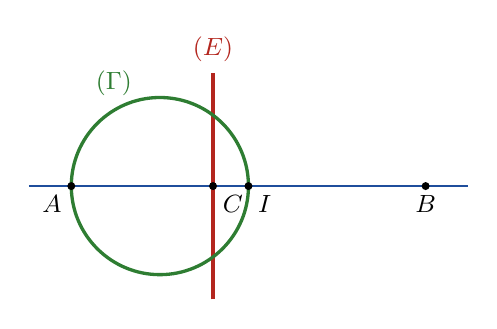
\begin{tikzpicture}[scale=0.9,font=\small]
\draw[cDef,thick] (-0.6,0)--(5.6,0);
\draw[cThm,very thick] (2,-1.6)--(2,1.6) node[above]{$(E)$};
\draw[cRem,very thick] (1.25,0) circle (1.25);
\fill (0,0) circle (1.6pt) node[below left]{$A$}; \fill (5,0) circle (1.6pt) node[below]{$B$};
\fill (2,0) circle (1.6pt) node[below right]{$C$}; \fill (2.5,0) circle (1.6pt) node[below right]{$I$};
\node[cRem] at (0.6,1.45){$(\Gamma)$};
\end{tikzpicture}
\end{LTR}}
\end{hal}

% ------------------------------------------------- 4
\begin{tamrin}{مجموعة النقط $MB=2MA$}
لتكن $A$ و $B$ نقطتين متمايزتين حيث $AB=6$ ، و $(E)$ مجموعة النقط $M$ من المستوي التي تحقق: $MB=2MA$.
\begin{enumerate}
\item برهن أنه من أجل كل نقطة $M$: \ $MB=2MA\iff\big(\V{MB}+2\V{MA}\big)\cdot\big(\V{MB}-2\V{MA}\big)=0$.
\item لتكن $I$ و $J$ نقطتين حيث: $2\V{IA}+\V{IB}=\vec0$ و $-2\V{JA}+\V{JB}=\vec0$.
\begin{sq}
\qa أنشئ النقطتين $I$ و $J$.
\qb أثبت أنه من أجل كل نقطة $M$: \ $\big(\V{MB}+2\V{MA}\big)\cdot\big(\V{MB}-2\V{MA}\big)=-3\,\V{MI}\cdot\V{MJ}$.
\end{sq}
\item عيّن ثم أنشئ المجموعة $(E)$.
\end{enumerate}
\end{tamrin}
\begin{hal}
\textbf{1.} الطولان موجبان ، إذن: $MB=2MA\iff MB^2=4MA^2\iff\V{MB}^2-\big(2\V{MA}\big)^2=0\iff\big(\V{MB}+2\V{MA}\big)\cdot\big(\V{MB}-2\V{MA}\big)=0$.
\QQ{2}
\begin{sq}
\qa $2\V{IA}+\V{IA}+\V{AB}=\vec0$ ، أي $3\V{AI}=\V{AB}$: \bx{\V{AI}=\dfrac13\V{AB}} \ ($AI=2$).\par
$-2\V{JA}+\V{JA}+\V{AB}=\vec0$ ، أي $\V{JA}=-\V{AB}$: \bx{\V{AJ}=-\V{AB}} \ ($J$ نظيرة $B$ بالنسبة إلى $A$).
\qb $I$ مرجح $\{(A;2);(B;1)\}$ ، إذن $\V{MB}+2\V{MA}=3\V{MI}$.\par
$J$ مرجح $\{(A;-2);(B;1)\}$ ، إذن $\V{MB}-2\V{MA}=(1-2)\V{MJ}=-\V{MJ}$.\par
ومنه: $\big(\V{MB}+2\V{MA}\big)\cdot\big(\V{MB}-2\V{MA}\big)=3\V{MI}\cdot\big(-\V{MJ}\big)=\bx{-3\,\V{MI}\cdot\V{MJ}}$.
\end{sq}
\QQ{3} $M\in(E)\iff-3\,\V{MI}\cdot\V{MJ}=0\iff\V{MI}\cdot\V{MJ}=0$.\par
\bx{(E)} \textbf{هي الدائرة التي قطرها $[IJ]$}: \ $IJ=IA+AJ=2+6=8$ ، فنصف قطرها $4$ ومركزها منتصف $[IJ]$ (النقطة $K$ حيث $\V{AK}=-\dfrac13\V{AB}$).
\RL{0.42}{%
\begin{molahada}[تصحيح]
المساواة $\V{MI}\cdot\V{MJ}=0$ تميّز \textbf{الدائرة ذات القطر $[IJ]$} ، وليس «المستقيم المحوري للقطعة $[IJ]$». \ تحقق: $I\in(E)$ لأن $IB=4=2\,IA$ ، و $J\in(E)$ لأن $JB=12=2\,JA$.
\end{molahada}}{0.55}{%
\begin{LTR}\centering
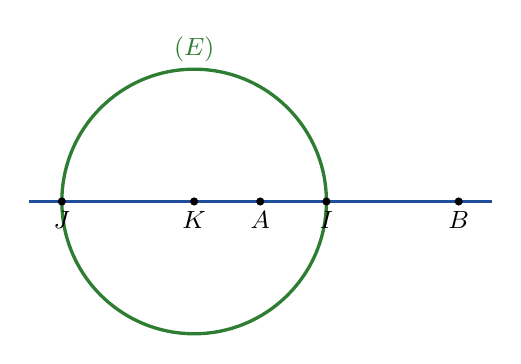
\begin{tikzpicture}[scale=0.42,font=\small]
\draw[cDef,thick] (-7,0)--(7,0);
\draw[cRem,very thick] (-2,0) circle (4);
\foreach \x/\n in {-6/J,0/A,2/I,6/B,-2/K} \fill (\x,0) circle (3.5pt) node[below]{$\n$};
\node[cRem] at (-2,4.6){$(E)$};
\end{tikzpicture}
\end{LTR}}
\end{hal}

% ------------------------------------------------- 5
\begin{tamrin}{مجموعة النقط $MA^2-MB^2=k$}
في معلم متعامد ومتجانس نعتبر النقطتين $A(1;0)$ و $B(4;0)$ ، فيكون $AB=3$.
\begin{enumerate}
\item بيّن أنه من أجل كل نقطة $M$: \ $MA^2-MB^2=2\,\V{AM}\cdot\V{AB}-9$.
\item عيّن مجموعة النقط $M$ التي تحقق: $MA^2-MB^2=-3$ ، ثم اكتب معادلة لها.
\end{enumerate}
\end{tamrin}
\begin{hal}
\textbf{1.}
\begin{align*}
MA^2-MB^2&=\V{MA}^2-\big(\V{MA}+\V{AB}\big)^2=\V{MA}^2-\V{MA}^2-2\,\V{MA}\cdot\V{AB}-\V{AB}^2\\
&=-2\,\V{MA}\cdot\V{AB}-AB^2=\bx{2\,\V{AM}\cdot\V{AB}-9}.
\end{align*}
\QQ{2} $MA^2-MB^2=-3\iff2\,\V{AM}\cdot\V{AB}=6\iff\V{AM}\cdot\V{AB}=3$.\par
لتكن $H$ المسقط العمودي لـ $M$ على $(AB)$: $\V{AH}\cdot\V{AB}=3$ ، و $H$ ثابتة ($AH=1$ في اتجاه $B$) ، فالمجموعة هي \textbf{المستقيم العمودي على $(AB)$ في $H(2;0)$}.\par
\textbf{تحليلياً:} $\V{AM}(x-1;y)$ و $\V{AB}(3;0)$: \ $3(x-1)+0\times y=3\iff\bx{x=2}$.
\end{hal}

% =====================================================================
\section{المستقيمات والدوائر في معلم متعامد ومتجانس}
% ------------------------------------------------- 6
\begin{tamrin}{دائرة ومماس}
المستوي منسوب إلى معلم متعامد ومتجانس $(O;\vec i,\vec j)$. نعتبر النقط: $A(1;-1)$ ، $B(1;3)$ ، $C(5;2)$ و $D(0;-2)$.
\begin{enumerate}
\item احسب مركبات الشعاعين $\V{AB}$ و $\V{AC}$ ، ثم احسب $\V{AB}\cdot\V{AC}$.
\item احسب $AB$ و $AC$ ثم استنتج $\cos\big(\V{AB};\V{AC}\big)$.
\item لتكن $(c)$ مجموعة النقط $M(x;y)$ التي تحقق: $x^2+y^2-2x-6y-3=0$. \ بيّن أن $(c)$ دائرة يطلب تعيين مركزها $\Omega$ ونصف قطرها $r$.
\item جد معادلة للمستقيم $(\Delta)$ الذي يشمل $D$ و $\vec n(3;2)$ شعاع ناظمي له.
\item
\begin{sq}
\qa بيّن أن المسافة بين $\Omega$ والمستقيم $(\Delta)$ هي $\sqrt{13}$.
\qb هل المستقيم $(\Delta)$ مماس للدائرة $(c)$؟ برّر.
\end{sq}
\end{enumerate}
\end{tamrin}
\begin{hal}
\textbf{1.} $\V{AB}(0;4)$ و $\V{AC}(4;3)$ ، ومنه $\V{AB}\cdot\V{AC}=0\times4+4\times3=\bx{12}$.
\QQ{2} $AB=\sqrt{0+16}=4$ ، $AC=\sqrt{16+9}=5$ ، و $\cos\big(\V{AB};\V{AC}\big)=\dfrac{\V{AB}\cdot\V{AC}}{AB\times AC}=\dfrac{12}{20}=\bx{\dfrac35}$.
\QQ{3} $x^2-2x+y^2-6y-3=0\iff(x-1)^2-1+(y-3)^2-9-3=0\iff(x-1)^2+(y-3)^2=13$.\par
$(c)$ دائرة مركزها \bx{\Omega(1;3)} ونصف قطرها \bx{r=\sqrt{13}}. \ (لاحظ أن $\Omega=B$).
\QQ{4} $(\Delta):3x+2y+c=0$ ، و $D\in(\Delta)$: $0-4+c=0$ ، أي $c=4$: \bx{(\Delta):3x+2y+4=0}.
\QQ{5}
\begin{sq}
\qa $d(\Omega;\Delta)=\dfrac{|3\times1+2\times3+4|}{\sqrt{9+4}}=\dfrac{13}{\sqrt{13}}=\bx{\sqrt{13}}$.
\qb $d(\Omega;\Delta)=r$ ، إذن \textbf{$(\Delta)$ مماس للدائرة $(c)$}. \ نقطة التماس هي المسقط العمودي لـ $\Omega$ على $(\Delta)$: $\Omega-\dfrac{13}{13}\vec n=(1-3;3-2)=(-2;1)$ ، وتحقق: $3(-2)+2(1)+4=0$ \ok.
\end{sq}
\end{hal}

% ------------------------------------------------- 7
\begin{tamrin}{مثلث قائم ودائرة}
المستوي منسوب إلى معلم متعامد ومتجانس $(O;\vec i,\vec j)$. لتكن النقط $A(-1;1)$ ، $B(-2;1)$ و $C(-1;-1)$.
\begin{enumerate}
\item احسب الجداء السلمي $\V{AB}\cdot\V{AC}$ ، ثم استنتج طبيعة المثلث $ABC$.
\item أوجد معادلة للمستقيم $(\Delta)$ الذي يشمل $A$ و $\V{BC}$ شعاع ناظمي له.
\item أوجد معادلة الدائرة $(c)$ التي مركزها $w(-1;3)$ ونصف قطرها $r=\sqrt5$.
\item تحقق أن $B$ تنتمي إلى الدائرة $(c)$.
\item احسب المسافة بين مركز الدائرة $(c)$ والمستقيم $(\Delta)$ ، ثم استنتج الوضع النسبي لـ $(c)$ و $(\Delta)$.
\end{enumerate}
\end{tamrin}
\begin{hal}
\textbf{1.} $\V{AB}(-1;0)$ و $\V{AC}(0;-2)$: \ $\V{AB}\cdot\V{AC}=0+0=\bx{0}$ ، إذن \textbf{$ABC$ قائم في $A$}.
\QQ{2} $\V{BC}(1;-2)$ ، فـ $(\Delta):x-2y+c=0$. \ $A\in(\Delta)$: $-1-2+c=0$ ، $c=3$: \bx{(\Delta):x-2y+3=0}.
\QQ{3} \bx{(c):(x+1)^2+(y-3)^2=5} ، أي $x^2+y^2+2x-6y+5=0$.
\QQ{4} $(-2+1)^2+(1-3)^2=1+4=5$ \ok ، إذن $B\in(c)$.
\QQ{5} $d(w;\Delta)=\dfrac{|-1-6+3|}{\sqrt{1+4}}=\bx{\dfrac{4}{\sqrt5}}\approx1{,}79$. \ وبما أن $\dfrac4{\sqrt5}<\sqrt5$ (لأن $4<5$) فإن \textbf{$(\Delta)$ يقطع $(c)$ في نقطتين}.
\end{hal}

% ------------------------------------------------- 8
\begin{tamrin}{الدائرة المحيطة بمثلث قائم وصورتها بتحاكٍ}
في معلم متعامد ومتجانس نعتبر النقط $A(2;0)$ ، $B(4;2)$ ، $C(-1;3)$ والمستقيم $(d):x+5y-21=0$.
\begin{enumerate}
\item احسب الجداء السلمي $\V{AB}\cdot\V{AC}$ ثم استنتج طبيعة المثلث $ABC$.
\item عيّن إحداثيي النقطة $D$ مركز الدائرة $(C)$ المحيطة بالمثلث $ABC$.
\item اكتب معادلة ديكارتية للدائرة $(C)$.
\item اكتب معادلة ديكارتية للمستقيم $(\Delta)$ المماس للدائرة $(C)$ في النقطة $B$ ، ثم تحقق أن $(\Delta)\perp(d)$.
\item احسب المسافة بين $D$ والمستقيم $(d)$ ، ثم ادرس وضعية $(d)$ بالنسبة إلى $(C)$.
\item عيّن صورة الدائرة $(C)$ بالتحاكي $h$ الذي مركزه $B$ ونسبته $2$.
\end{enumerate}
\end{tamrin}
\begin{hal}
\textbf{1.} $\V{AB}(2;2)$ و $\V{AC}(-3;3)$: \ $\V{AB}\cdot\V{AC}=-6+6=\bx{0}$ ، فـ \textbf{$ABC$ قائم في $A$}.
\QQ{2} مركز الدائرة المحيطة بمثلث قائم هو منتصف الوتر $[BC]$: \ $D\Big(\dfrac{4-1}{2};\dfrac{2+3}{2}\Big)$ ، أي \bx{D\Big(\dfrac32;\dfrac52\Big)}.
\QQ{3} $r^2=DB^2=\Big(4-\dfrac32\Big)^2+\Big(2-\dfrac52\Big)^2=\dfrac{25}4+\dfrac14=\dfrac{13}{2}$: \ \bx{(C):\Big(x-\dfrac32\Big)^2+\Big(y-\dfrac52\Big)^2=\dfrac{13}{2}}.
\QQ{4} $\V{DB}\Big(\dfrac52;-\dfrac12\Big)$ ناظمي لـ $(\Delta)$ ، أو $\vec n(5;-1)$: \ $(\Delta):5x-y+c=0$ ، و $B\in(\Delta)$: $20-2+c=0$ ، $c=-18$.\par
\bx{(\Delta):5x-y-18=0} \ (وهي نفسها $\dfrac52x-\dfrac12y-9=0$).\par
شعاع ناظمي لـ $(d)$ هو $\vec n'(1;5)$ ، و $\vec n\cdot\vec n'=5-5=0$: الناظميان متعامدان ، إذن \textbf{$(\Delta)\perp(d)$}.
\QQ{5} $d(D;(d))=\dfrac{\big|\frac32+\frac{25}2-21\big|}{\sqrt{1+25}}=\dfrac{|-7|}{\sqrt{26}}=\bx{\dfrac{7}{\sqrt{26}}}$ ، و $r=\sqrt{\dfrac{13}2}=\dfrac{\sqrt{26}}{2}=\dfrac{13}{\sqrt{26}}$.\par
$\dfrac7{\sqrt{26}}<\dfrac{13}{\sqrt{26}}$ ، إذن \textbf{$(d)$ يقطع $(C)$ في نقطتين}.
\QQ{6} صورة $(C)$ هي الدائرة $(C')$ التي مركزها $D'=h(D)$ ونصف قطرها $r'=|2|\,r=\sqrt{26}$.\par
$\V{BD'}=2\V{BD}=2\Big(-\dfrac52;\dfrac12\Big)=(-5;1)$ ، إذن $D'(-1;3)=C$. \quad \bx{(C'):(x+1)^2+(y-3)^2=26}.
\end{hal}

% ------------------------------------------------- 9
\begin{tamrin}{تقاطع مستقيم ودائرة ومساحة مثلث}
في معلم متعامد ومتجانس نعتبر النقطتين $A(1;2)$ ، $B(0;5)$ والدائرة $(C):x^2+y^2-2x-3=0$.
\begin{enumerate}
\item اكتب معادلة ديكارتية للمستقيم $(D)$ الذي يشمل $I(-1;1)$ و $\vec u(2;1)$ شعاع توجيه له.
\item حدّد المركز $\Omega$ ونصف القطر $r$ للدائرة $(C)$ ، ثم تحقق أن $A\in(C)$.
\item اكتب معادلة ديكارتية للمستقيم $(\Delta)$ المار من $B$ و $\vec n(3;4)$ شعاع ناظمي له.
\item بيّن أن تقاطع $(\Delta)$ مع $(C)$ مجموعة خالية.
\item تحقق أن $(C)$ و $(D)$ يتقاطعان في نقطتين ، الأولى هي $A$ والثانية نرمز لها بـ $F$.
\item احسب مساحة المثلث $A\Omega F$ إذا علمت أن $\sin\widehat{A\Omega F}=0{,}8$.
\item احسب المسافة بين $\Omega$ والمستقيم $(D)$ بطريقتين.
\end{enumerate}
\end{tamrin}
\begin{hal}
\textbf{1.} $\vec u(2;1)$ توجيه ، فـ $\vec n(1;-2)$ ناظمي: $(D):x-2y+c=0$ ، و $I\in(D)$: $-1-2+c=0$: \bx{(D):x-2y+3=0}.
\QQ{2} $(x-1)^2-1+y^2-3=0\iff(x-1)^2+y^2=4$: \bx{\Omega(1;0)} و \bx{r=2}. \ $(1-1)^2+2^2=4$ \ok ، إذن $A\in(C)$.
\QQ{3} $(\Delta):3x+4y+c=0$ ، و $B\in(\Delta)$: $20+c=0$: \bx{(\Delta):3x+4y-20=0}.
\QQ{4} $d(\Omega;\Delta)=\dfrac{|3+0-20|}{\sqrt{9+16}}=\dfrac{17}{5}=3{,}4>2=r$ ، إذن \bx{(\Delta)\cap(C)=\varnothing}.\par
{\small (يمكن أيضاً التعويض: نحصل على معادلة من الدرجة الثانية مميزها سالب.)}
\QQ{5} من $(D)$: $x=2y-3$. نعوّض في $(C)$: $(2y-4)^2+y^2=4\iff5y^2-16y+12=0$.\par
$\Delta'=64-60=4$: \ $y_1=\dfrac{8+2}{5}=2$ و $y_2=\dfrac{8-2}5=\dfrac65$.\par
$y=2\Rightarrow x=1$: النقطة $A(1;2)$. \quad $y=\dfrac65\Rightarrow x=-\dfrac35$: \ \bx{F\Big(-\dfrac35;\dfrac65\Big)}.
\QQ{6} $\Omega A=\Omega F=r=2$: \ $S=\dfrac12\,\Omega A\times\Omega F\times\sin\widehat{A\Omega F}=\dfrac12\times2\times2\times0{,}8=\bx{1{,}6}$.
\QQ{7} \textbf{الطريقة الأولى:} $d(\Omega;D)=\dfrac{|1-0+3|}{\sqrt{1+4}}=\bx{\dfrac4{\sqrt5}}\approx1{,}79$.\par
\textbf{الطريقة الثانية:} ليكن $H$ المسقط العمودي لـ $\Omega$ على $(AF)=(D)$: \ $S=\dfrac{\Omega H\times AF}{2}$.\par
$AF=\sqrt{\Big(\dfrac85\Big)^2+\Big(\dfrac45\Big)^2}=\sqrt{\dfrac{80}{25}}=\dfrac{4}{\sqrt5}$ ، ومنه $\Omega H=\dfrac{2S}{AF}=\dfrac{3{,}2}{4/\sqrt5}=\dfrac{4\sqrt5}{5}=\dfrac4{\sqrt5}$ \ok.
\end{hal}

% ------------------------------------------------- 10
\begin{tamrin}{دائرة ومماسان متوازيان}
المستوي منسوب إلى معلم متعامد ومتجانس $(O;\vec i,\vec j)$. نعتبر النقط $B\big(0;\sqrt3\big)$ ، $C\big(0;-\sqrt3\big)$ و $M(x;y)$.
\begin{enumerate}
\item بيّن أن مجموعة النقط $M$ من المستوي التي تحقق $\V{MB}\cdot\V{MC}=0$ هي الدائرة $(C)$ ، يطلب تحديد مركزها ونصف قطرها.
\item اكتب معادلة المستقيمين $(T_1)$ و $(T_2)$ مماسي الدائرة $(C)$ في النقطتين $C$ و $B$ على الترتيب.
\item بيّن أن $(T_1)$ يوازي $(T_2)$.
\item ارسم الدائرة $(C)$ والمستقيمين $(T_1)$ و $(T_2)$.
\end{enumerate}
\end{tamrin}
\begin{hal}
\textbf{1.} $\V{MB}\big(-x;\sqrt3-y\big)$ و $\V{MC}\big(-x;-\sqrt3-y\big)$:
\[\V{MB}\cdot\V{MC}=(-x)(-x)+\big(\sqrt3-y\big)\big(-\sqrt3-y\big)=x^2+y^2-3.\]
$\V{MB}\cdot\V{MC}=0\iff x^2+y^2=3=\big(\sqrt3\big)^2$: \ $(C)$ دائرة مركزها \bx{O(0;0)} ونصف قطرها \bx{r=\sqrt3} (الدائرة ذات القطر $[BC]$).
\RL{0.6}{%
\QQ{2} المماس في $C$ عمودي على $\V{OC}\big(0;-\sqrt3\big)$:\par
$M\in(T_1)\iff\V{CM}\cdot\V{OC}=0\iff0\times x-\sqrt3\big(y+\sqrt3\big)=0$ ، أي \bx{(T_1):y=-\sqrt3}.\par
بنفس الطريقة: $\V{BM}\cdot\V{OB}=0\iff\sqrt3\big(y-\sqrt3\big)=0$ ، أي \bx{(T_2):y=\sqrt3}.
\QQ{3} المستقيمان من الشكل $y=k$ ، أي كلاهما يوازي محور الفواصل ، إذن \textbf{$(T_1)\parallel(T_2)$}.\par
(أو: لهما نفس الشعاع الناظمي $\vec j$.)
\QQ{4} الرسم مقابل.}{0.37}{%
\begin{LTR}\centering
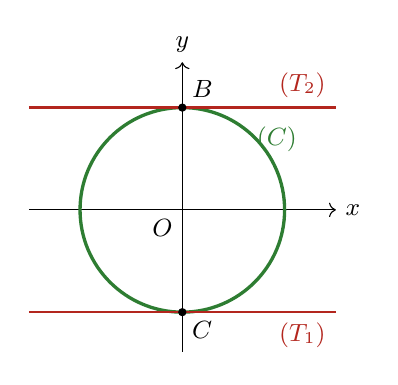
\begin{tikzpicture}[scale=0.75,font=\small]
\draw[->] (-2.6,0)--(2.6,0) node[right]{$x$}; \draw[->] (0,-2.4)--(0,2.5) node[above]{$y$};
\draw[cRem,very thick] (0,0) circle (1.732);
\draw[cThm,thick] (-2.6,1.732)--(2.6,1.732) node[above left]{$(T_2)$};
\draw[cThm,thick] (-2.6,-1.732)--(2.6,-1.732) node[below left]{$(T_1)$};
\fill (0,1.732) circle (2pt) node[above right]{$B$}; \fill (0,-1.732) circle (2pt) node[below right]{$C$};
\node[below left] at (0,0){$O$}; \node[cRem] at (1.6,1.2){$(C)$};
\end{tikzpicture}
\end{LTR}}
\end{hal}

% ------------------------------------------------- 11
\begin{tamrin}{مستقيمان متعامدان ومجموعة نقط}
في معلم متعامد ومتجانس $(O;\vec i,\vec j)$ ، ليكن $(D)$ المستقيم الذي معادلته: $3x+3y-5=0$.
\begin{enumerate}
\item اكتب معادلة للمستقيم $(\Delta)$ الذي يشمل $A(-1;2)$ ويعامد $(D)$.
\item عيّن إحداثيي النقطة $B$ نقطة تقاطع المستقيمين $(D)$ و $(\Delta)$ ، ثم احسب $AB$.
\item عيّن مجموعة النقط $M(x;y)$ من المستوي التي تحقق: $\V{MA}\cdot\V{MB}=AB$.
\end{enumerate}
\end{tamrin}
\begin{hal}
\textbf{1.} $\vec n(3;3)$ ناظمي لـ $(D)$ ، فهو شعاع توجيه لـ $(\Delta)$. \ $M\in(\Delta)\iff\V{AM}\cdot\vec u=0$ حيث $\vec u(-3;3)$ توجيه لـ $(D)$:\par
$-3(x+1)+3(y-2)=0\iff-3x+3y-9=0$ ، أي \bx{(\Delta):x-y+3=0}.
\QQ{2} نحل الجملة $\begin{cases}3x+3y-5=0\\x-y+3=0\end{cases}$: \ من الثانية $x=y-3$ ، نعوّض: $3(y-3)+3y-5=0\iff6y=14\iff y=\dfrac73$ ، و $x=\dfrac73-3=-\dfrac23$.\par
\bx{B\Big(-\dfrac23;\dfrac73\Big)} \ (تحقق: $-2+7-5=0$ \ok \ و \ $-\dfrac23-\dfrac73+3=0$ \ok).\par
$\V{AB}\Big(\dfrac13;\dfrac13\Big)$ ، إذن $AB=\sqrt{\dfrac19+\dfrac19}=\bx{\dfrac{\sqrt2}{3}}$.
\QQ{3} لتكن $K$ منتصف $[AB]$: \ $K\Big(-\dfrac56;\dfrac{13}6\Big)$ ، و $\V{MA}\cdot\V{MB}=MK^2-\dfrac{AB^2}{4}=MK^2-\dfrac1{18}$.\par
$\V{MA}\cdot\V{MB}=AB\iff MK^2=\dfrac{\sqrt2}{3}+\dfrac1{18}=\dfrac{6\sqrt2+1}{18}$.\par
المجموعة هي \textbf{الدائرة التي مركزها $K\Big(-\dfrac56;\dfrac{13}6\Big)$ ونصف قطرها} \bx{\sqrt{\dfrac{6\sqrt2+1}{18}}\approx0{,}726}:
\[\Big(x+\dfrac56\Big)^2+\Big(y-\dfrac{13}6\Big)^2=\dfrac{6\sqrt2+1}{18}.\]
\begin{molahada}[تصحيح]
عند حل الجملة يجب أن نحصل على $B\Big(-\dfrac23;\dfrac73\Big)$ ، لا على $B\Big(\dfrac73;-\dfrac23\Big)$: هذه الأخيرة تحقق معادلة $(D)$ لكنها لا تحقق معادلة $(\Delta)$ ($\dfrac73+\dfrac23+3=6\ne0$). \ لذلك $AB=\dfrac{\sqrt2}{3}$ (لا $\dfrac23\sqrt{41}$) ، ومركز الدائرة هو منتصف $[AB]$ أي $K\Big(-\dfrac56;\dfrac{13}6\Big)$.
\end{molahada}
\end{hal}

% ------------------------------------------------- 12
\begin{tamrin}{دائرة ، مماس ونظيرة}
المستوي منسوب إلى معلم متعامد ومتجانس $(O;\vec i,\vec j)$. لتكن $(C)$ مجموعة النقط $M(x;y)$ المعرّفة بـ: $\dfrac12\big(x^2+y^2\big)-3x+y+\dfrac52=0$.
\begin{enumerate}
\item
\begin{sq}
\qa بيّن أن $(C)$ دائرة يطلب تحديد إحداثيي مركزها $\Omega$ ونصف قطرها.
\qb أثبت أن النقطة $A(1;-2)$ من $(C)$.
\end{sq}
\item اكتب معادلة المستقيم $(T)$ مماس الدائرة $(C)$ عند النقطة $A$.
\item لتكن $B$ نظيرة $\Omega$ بالنسبة إلى $A$.
\begin{sq}
\qa عيّن إحداثيي النقطة $B$.
\qb اكتب معادلة الدائرة $(C')$ التي مركزها $B$ والمماسة لـ $(C)$ عند النقطة $A$.
\end{sq}
\item ادرس الوضع النسبي بين المستقيم $(D):6x+2y-5=0$ والدائرة $(C)$.
\end{enumerate}
\end{tamrin}
\begin{hal}
\textbf{1.}
\begin{sq}
\qa بضرب الطرفين في $2$: $x^2+y^2-6x+2y+5=0\iff(x-3)^2-9+(y+1)^2-1+5=0\iff(x-3)^2+(y+1)^2=5$.\par
$(C)$ دائرة مركزها \bx{\Omega(3;-1)} ونصف قطرها \bx{r=\sqrt5}.
\qb $(1-3)^2+(-2+1)^2=4+1=5$ \ok ، إذن $A\in(C)$.
\end{sq}
\QQ{2} $M\in(T)\iff\V{AM}\cdot\V{\Omega A}=0$ ، مع $\V{\Omega A}(-2;-1)$:\par
$-2(x-1)-(y+2)=0\iff-2x-y=0$ ، أي \bx{(T):2x+y=0}.
\QQ{3}
\begin{sq}
\qa $A$ منتصف $[\Omega B]$: \ $x_B=2x_A-x_\Omega=2-3=-1$ و $y_B=2y_A-y_\Omega=-4+1=-3$: \bx{B(-1;-3)}.
\qb $(C')$ تمر بـ $A$ ، فنصف قطرها $BA=\Omega A=\sqrt5$: \ \bx{(C'):(x+1)^2+(y+3)^2=5}.\par
المركزان $\Omega$ و $B$ و $A$ على استقامة واحدة ، و $(T)$ عمودي على $(\Omega B)$ في $A$: فهو مماس مشترك ، و $(C)$ و $(C')$ متماستان في $A$.
\end{sq}
\QQ{4} $d(\Omega;D)=\dfrac{|6\times3+2\times(-1)-5|}{\sqrt{36+4}}=\dfrac{11}{\sqrt{40}}\approx1{,}74<\sqrt5\approx2{,}24$: \ \textbf{$(D)$ يقطع $(C)$ في نقطتين}.
\end{hal}

% ------------------------------------------------- 13
\begin{tamrin}{مسألة شاملة: مماس ، جداء سلمي ومجموعات نقط}
المستوي منسوب إلى معلم متعامد ومتجانس $(O;\vec i,\vec j)$ حيث $\nV{\vec i}=\nV{\vec j}=1\,cm$. \ لتكن النقط $A(2;1)$ ، $B(5;-1)$ و $C(8;3)$ ، و $H$ منتصف القطعة $[AC]$.
\begin{enumerate}
\item علّم النقط $A$ ، $B$ ، $C$ و $H$ ، ثم اكتب معادلة ديكارتية للمستقيم $(\Delta)$ الذي يشمل $A$ و $\vec v(3;-2)$ ناظمي له.
\item لتكن $(\gamma)$ مجموعة النقط $M(x;y)$ حيث: $x^2+y^2-10x+2y+13=0$.
\begin{sq}
\qa أثبت أن $(\gamma)$ دائرة مركزها $B$ ونصف قطرها $R$ يطلب تعيينه.
\qb أنشئ المستقيم $(\Delta)$ والدائرة $(\gamma)$.
\qc تحقق حسابياً أن $A\in(\gamma)$ ، ثم حدّد بدقة المسافة $d(B;\Delta)$.
\qd استنتج الوضعية النسبية لـ $(\Delta)$ و $(\gamma)$.
\end{sq}
\item احسب الجداء السلمي $\V{BA}\cdot\V{BC}$ بطريقتين ، واستنتج قيمة مقرّبة بالدرجات لقيس الزاوية $\widehat{ABC}$.
\item احسب الطول $BH$ بطريقتين مختلفتين.
\item حدّد طبيعة وعناصر $(E)$ مجموعة النقط $N$ من المستوي التي تحقق: $NA^2+NC^2=21$.
\item حدّد طبيعة وعناصر $(F)$ مجموعة النقط $M$ التي تحقق: $\V{MA}\cdot\V{MC}=0$ ، واكتب معادلة ديكارتية لها.
\item ليكن $h$ التحاكي الذي مركزه $O(0;0)$ ونسبته $-\dfrac12$ ، و $(\gamma')$ صورة الدائرة $(\gamma)$ بالتحاكي $h$.
\begin{sq}
\qa اكتب معادلة ديكارتية للدائرة $(\gamma')$.
\qb استنتج محيط ومساحة الدائرة $(\gamma')$.
\end{sq}
\end{enumerate}
\end{tamrin}
\begin{hal}
\RL{0.56}{%
\textbf{1.} $H\Big(\dfrac{2+8}2;\dfrac{1+3}2\Big)=H(5;2)$.\par
$(\Delta):3x-2y+c=0$ ، و $A\in(\Delta)$: $6-2+c=0$ ، $c=-4$:\par
\bx{(\Delta):3x-2y-4=0}.
\QQ{2}
\begin{sq}
\qa $(x-5)^2-25+(y+1)^2-1+13=0$ ، أي\par $(x-5)^2+(y+1)^2=13$:\par
مركزها \bx{B(5;-1)} ونصف قطرها \bx{R=\sqrt{13}}.
\qb الرسم مقابل.
\end{sq}}{0.41}{%
\begin{LTR}\centering
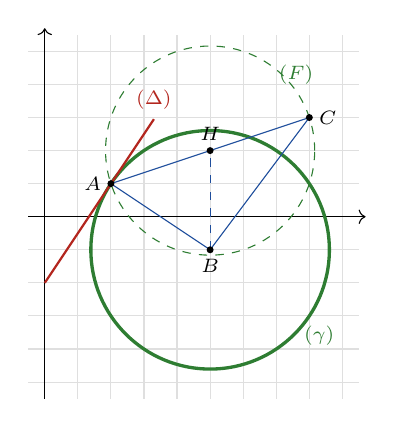
\begin{tikzpicture}[scale=0.42,font=\scriptsize]
\draw[gray!25] (-0.5,-5.5) grid (9.5,5.5);
\draw[->] (-0.5,0)--(9.7,0); \draw[->] (0,-5.5)--(0,5.7);
\draw[cRem,very thick] (5,-1) circle (3.606);
\draw[cRem,dashed] (5,2) circle (3.162);
\draw[cThm,thick] (0,-2)--(3.3,2.95) node[above]{$(\Delta)$};
\draw[cDef] (2,1)--(5,-1)--(8,3)--cycle; \draw[cDef,dashed] (5,-1)--(5,2);
\foreach \p/\n/\a in {{(2,1)}/A/left,{(5,-1)}/B/below,{(8,3)}/C/right,{(5,2)}/H/above}\fill \p circle (3pt) node[\a]{$\n$};
\node[cRem] at (8.3,-3.6){$(\gamma)$}; \node[cRem] at (7.6,4.3){$(F)$};
\end{tikzpicture}
\end{LTR}}
\begin{sq}
\qc $(2-5)^2+(1+1)^2=9+4=13$ \ok ، إذن $A\in(\gamma)$. \quad $d(B;\Delta)=\dfrac{|15+2-4|}{\sqrt{9+4}}=\dfrac{13}{\sqrt{13}}=\bx{\sqrt{13}}$.
\qd $d(B;\Delta)=R$: \textbf{$(\Delta)$ مماس للدائرة $(\gamma)$ في النقطة $A$} (لأن $A$ مشتركة بينهما).
\end{sq}
\QQ{3} \textbf{الطريقة 1 (تحليلياً):} $\V{BA}(-3;2)$ و $\V{BC}(3;4)$: \ $\V{BA}\cdot\V{BC}=-9+8=\bx{-1}$.\par
\textbf{الطريقة 2 (بالمنتصف $H$):} $\V{BA}\cdot\V{BC}=BH^2-\dfrac{AC^2}{4}$ ، مع $BH=3$ و $AC^2=36+4=40$: \ $9-10=-1$ \ok.\par
$\cos\widehat{ABC}=\dfrac{-1}{BA\times BC}=\dfrac{-1}{\sqrt{13}\times5}\approx-0{,}0555$ ، إذن \bx{\widehat{ABC}\approx93{,}18^\circ}.
\QQ{4} \textbf{الطريقة 1:} $\V{BH}(0;3)$ ، إذن \bx{BH=3}.\par
\textbf{الطريقة 2 (مبرهنة المتوسط):} $BA^2+BC^2=2BH^2+\dfrac{AC^2}2$ ، أي $13+25=2BH^2+20$ ، ومنه $BH^2=9$ و $BH=3$ \ok.
\QQ{5} $NA^2+NC^2=2NH^2+\dfrac{AC^2}{2}=2NH^2+20$. \ $NA^2+NC^2=21\iff NH^2=\dfrac12\iff NH=\dfrac{\sqrt2}2$.\par
$(E)$ \textbf{دائرة مركزها $H(5;2)$ ونصف قطرها} \bx{\dfrac{\sqrt2}{2}}.
\QQ{6} $(F)$ \textbf{هي الدائرة التي قطرها $[AC]$}: مركزها $H(5;2)$ ونصف قطرها $\dfrac{AC}2=\dfrac{\sqrt{40}}2=\sqrt{10}$.\par
تحليلياً: $(2-x)(8-x)+(1-y)(3-y)=0\iff x^2+y^2-10x-4y+19=0\iff\bx{(x-5)^2+(y-2)^2=10}$.
\QQ{7}
\begin{sq}
\qa $(\gamma')$ مركزها $B'=h(B)$: $\V{OB'}=-\dfrac12\V{OB}$ ، أي $B'\Big(-\dfrac52;\dfrac12\Big)$ ، ونصف قطرها $R'=\Big|-\dfrac12\Big|R=\dfrac{\sqrt{13}}2$:
\[(\gamma'):\Big(x+\dfrac52\Big)^2+\Big(y-\dfrac12\Big)^2=\dfrac{13}{4}.\]
\qb المحيط: $P'=2\pi R'=\bx{\pi\sqrt{13}\ cm}\approx11{,}33\,cm$. \quad المساحة: $S'=\pi R'^2=\bx{\dfrac{13\pi}{4}\ cm^2}\approx10{,}21\,cm^2$.
\end{sq}
\end{hal}

% =====================================================================
\section{دساتير الجمع والمعادلات المثلثية}
% ------------------------------------------------- 14
\begin{tamrin}{حساب قيم مضبوطة}
\begin{enumerate}
\item إذا علمت أن $\sin\Big(\dfrac{7\pi}{12}\Big)=\dfrac{\sqrt2+\sqrt6}{4}$ ، احسب $\sin\Big(\dfrac{5\pi}{12}\Big)$ بطريقتين مختلفتين.
\item احسب $\cos\Big(\dfrac{5\pi}{12}\Big)$ ، ثم استنتج أن $\tan\Big(\dfrac{5\pi}{12}\Big)=2+\sqrt3$.
\item باستعمال دستور التضعيف ، احسب $\cos\Big(\dfrac{\pi}{8}\Big)$ و $\sin\Big(\dfrac{\pi}{8}\Big)$.
\end{enumerate}
\end{tamrin}
\begin{hal}
\textbf{1.} \textbf{الطريقة 1:} $\dfrac{5\pi}{12}=\pi-\dfrac{7\pi}{12}$ ، و $\sin(\pi-a)=\sin a$: \ $\sin\dfrac{5\pi}{12}=\sin\dfrac{7\pi}{12}=\bx{\dfrac{\sqrt2+\sqrt6}{4}}$.\par
\textbf{الطريقة 2:} $\dfrac{5\pi}{12}=\dfrac{\pi}4+\dfrac{\pi}6$:
\[\sin\dfrac{5\pi}{12}=\sin\dfrac\pi4\cos\dfrac\pi6+\cos\dfrac\pi4\sin\dfrac\pi6=\dfrac{\sqrt2}2\cdot\dfrac{\sqrt3}2+\dfrac{\sqrt2}2\cdot\dfrac12=\dfrac{\sqrt6+\sqrt2}{4}\ \text{\ok}.\]
\QQ{2} $\cos\dfrac{5\pi}{12}=\cos\dfrac\pi4\cos\dfrac\pi6-\sin\dfrac\pi4\sin\dfrac\pi6=\dfrac{\sqrt6}4-\dfrac{\sqrt2}4=\bx{\dfrac{\sqrt6-\sqrt2}{4}}$.
\[\tan\dfrac{5\pi}{12}=\dfrac{\sqrt6+\sqrt2}{\sqrt6-\sqrt2}=\dfrac{\big(\sqrt6+\sqrt2\big)^2}{6-2}=\dfrac{8+2\sqrt{12}}{4}=\dfrac{8+4\sqrt3}{4}=\bx{2+\sqrt3}.\]
\QQ{3} $\cos^2\dfrac\pi8=\dfrac{1+\cos\frac\pi4}{2}=\dfrac{2+\sqrt2}{4}$ ، و $\cos\dfrac\pi8>0$: \ \bx{\cos\dfrac\pi8=\dfrac{\sqrt{2+\sqrt2}}{2}}.\par
$\sin^2\dfrac\pi8=\dfrac{1-\cos\frac\pi4}{2}=\dfrac{2-\sqrt2}{4}$ ، و $\sin\dfrac\pi8>0$: \ \bx{\sin\dfrac\pi8=\dfrac{\sqrt{2-\sqrt2}}{2}}.
\end{hal}

% ------------------------------------------------- 15
\begin{tamrin}{متطابقات مثلثية}
برهن أنه من أجل كل عدد حقيقي $x$:
\begin{sq}
\qa $\cos^4x-\sin^4x=\cos2x$
\qb $\big(\sin x+\cos x\big)^2=1+\sin2x$
\qc $\sin3x=3\sin x-4\sin^3x$
\qd $\cos3x=4\cos^3x-3\cos x$
\end{sq}
\end{tamrin}
\begin{hal}
\begin{sq}
\qa $\cos^4x-\sin^4x=\big(\cos^2x-\sin^2x\big)\big(\cos^2x+\sin^2x\big)=\cos2x\times1=\cos2x$.
\qb $\big(\sin x+\cos x\big)^2=\sin^2x+\cos^2x+2\sin x\cos x=1+\sin2x$.
\qc $\sin3x=\sin(2x+x)=\sin2x\cos x+\cos2x\sin x=2\sin x\cos^2x+\big(1-2\sin^2x\big)\sin x$\par
$=2\sin x\big(1-\sin^2x\big)+\sin x-2\sin^3x=3\sin x-4\sin^3x$.
\qd $\cos3x=\cos2x\cos x-\sin2x\sin x=\big(2\cos^2x-1\big)\cos x-2\sin^2x\cos x$\par
$=2\cos^3x-\cos x-2\big(1-\cos^2x\big)\cos x=4\cos^3x-3\cos x$.
\end{sq}
\end{hal}

% ------------------------------------------------- 16
\begin{tamrin}{معادلات من الشكل $a\cos x+b\sin x=c$}
\begin{enumerate}
\item حل في المجال $]-\pi;\pi]$ المعادلة: $\cos x+\sin x=1$.
\item حل في $\R$ المعادلة: $\sqrt3\cos x-\sin x=\sqrt2$.
\item حل في $\R$ المعادلة: $\cos4x=\dfrac{1}{\sqrt2}$.
\end{enumerate}
\end{tamrin}
\begin{hal}
\textbf{1.} $\sqrt{1^2+1^2}=\sqrt2$: \ $\cos x+\sin x=\sqrt2\Big(\dfrac{\sqrt2}2\cos x+\dfrac{\sqrt2}2\sin x\Big)=\sqrt2\cos\Big(x-\dfrac\pi4\Big)$.\par
$\cos\Big(x-\dfrac\pi4\Big)=\dfrac1{\sqrt2}=\cos\dfrac\pi4\iff x-\dfrac\pi4=\dfrac\pi4+2k\pi$ \ أو \ $x-\dfrac\pi4=-\dfrac\pi4+2k\pi$ ، $k\in\Z$.\par
أي $x=\dfrac\pi2+2k\pi$ أو $x=2k\pi$. \ في $]-\pi;\pi]$: \ \bx{S=\Big\{0;\dfrac\pi2\Big\}} \ (تحقق: $1+0=1$ ، $0+1=1$ \ok).
\QQ{2} $\sqrt{3+1}=2$: \ $\sqrt3\cos x-\sin x=2\Big(\dfrac{\sqrt3}2\cos x-\dfrac12\sin x\Big)=2\cos\Big(x+\dfrac\pi6\Big)$.\par
$\cos\Big(x+\dfrac\pi6\Big)=\dfrac{\sqrt2}2=\cos\dfrac\pi4\iff x+\dfrac\pi6=\pm\dfrac\pi4+2k\pi$:
\[\bx{x=\dfrac{\pi}{12}+2k\pi}\quad\text{\ar{أو}}\quad\bx{x=-\dfrac{5\pi}{12}+2k\pi}\ ,\ k\in\Z.\]
\QQ{3} $\cos4x=\cos\dfrac\pi4\iff4x=\pm\dfrac\pi4+2k\pi\iff\bx{x=\pm\dfrac{\pi}{16}+\dfrac{k\pi}{2}}$ ، $k\in\Z$.
\end{hal}

% =====================================================================
\section{اختيار من متعدد ، صحيح أم خطأ}
% ------------------------------------------------- 17
\begin{tamrin}{اختيار من متعدد}
اختر الإجابة الصحيحة الوحيدة مع التعليل (المعلم متعامد ومتجانس):
\begin{enumerate}
\item إذا كان $\vec u(2;-1)$ و $\vec v(3;4)$ فإن $\vec u\cdot\vec v$ يساوي:
\ABC{$2$}{$10$}{$-2$}
\item $\nV{\vec u}=3$ ، $\nV{\vec v}=2$ و $(\vec u;\vec v)=\dfrac{2\pi}{3}$ ، إذن $\vec u\cdot\vec v$ يساوي:
\ABC{$3$}{$-3$}{$-3\sqrt3$}
\item المسافة بين المبدأ $O$ والمستقيم $3x-4y+10=0$ هي:
\ABC{$10$}{$2$}{$\dfrac{10}{7}$}
\item الدائرة $x^2+y^2+4x-6y+4=0$ مركزها ونصف قطرها:
\ABC{$(2;-3)$ ، $3$}{$(-2;3)$ ، $9$}{$(-2;3)$ ، $3$}
\item $\cos\dfrac{\pi}{12}$ يساوي:
\ABC{$\dfrac{\sqrt6+\sqrt2}{4}$}{$\dfrac{\sqrt6-\sqrt2}{4}$}{$\dfrac{\sqrt3}{4}$}
\item $A$ و $B$ نقطتان متمايزتان. مجموعة النقط $M$ حيث $\V{MA}\cdot\V{MB}=0$ هي:
\ABC{محور $[AB]$}{المستقيم $(AB)$}{الدائرة ذات القطر $[AB]$}
\item $ABC$ مثلث فيه $AB=5$ ، $AC=3$ و $\widehat{A}=\dfrac{2\pi}{3}$ ، إذن $BC$ يساوي:
\ABC{$7$}{$\sqrt{19}$}{$49$}
\item المستقيم الذي يشمل $A(1;1)$ و $\vec n(2;-3)$ ناظمي له معادلته:
\ABC{$3x+2y-5=0$}{$2x-3y+1=0$}{$2x-3y-1=0$}
\end{enumerate}
\end{tamrin}
\begin{hal}
\textbf{1.} (أ): $6-4=2$. \quad \textbf{2.} (ب): $3\times2\times\cos\dfrac{2\pi}3=6\times\Big(-\dfrac12\Big)=-3$.
\QQ{3} (ب): $\dfrac{|10|}{\sqrt{9+16}}=\dfrac{10}5=2$.
\QQ{4} (جـ): $(x+2)^2-4+(y-3)^2-9+4=0\iff(x+2)^2+(y-3)^2=9$ ، فالمركز $(-2;3)$ ونصف القطر $3$ (وليس $9$).
\QQ{5} (أ): $\cos\Big(\dfrac\pi3-\dfrac\pi4\Big)=\dfrac12\cdot\dfrac{\sqrt2}2+\dfrac{\sqrt3}2\cdot\dfrac{\sqrt2}2=\dfrac{\sqrt2+\sqrt6}4$.
\QQ{6} (جـ): $\V{MA}\perp\V{MB}$ أو $M\in\{A;B\}$.
\QQ{7} (أ): الكاشي: $BC^2=25+9-2\times5\times3\times\Big(-\dfrac12\Big)=49$ ، $BC=7$.
\QQ{8} (ب): $2x-3y+c=0$ و $2-3+c=0$ ، $c=1$.
\end{hal}

% ------------------------------------------------- 18
\begin{tamrin}{صحيح أم خطأ}
أجب بصحيح أو خطأ مع التعليل:
\begin{enumerate}
\item إذا كان $\vec u\cdot\vec v=0$ فإن $\vec u=\vec0$ أو $\vec v=\vec0$.
\item $\nV{\vec u+\vec v}^2=\nV{\vec u}^2+\nV{\vec v}^2$ إذا وفقط إذا كان $\vec u\perp\vec v$.
\item المستقيمان $2x-y+1=0$ و $x+2y-3=0$ متعامدان.
\item المعادلة $x^2+y^2-2x+4y+6=0$ هي معادلة دائرة.
\item من أجل كل عدد حقيقي $x$: \ $\cos2x=1-2\cos^2x$.
\item من أجل كل عدد حقيقي $x$: \ $\sqrt3\cos x+\sin x=2\cos\Big(x-\dfrac\pi6\Big)$.
\item إذا كان $\V{AB}\cdot\V{AC}<0$ فإن الزاوية $\widehat{BAC}$ منفرجة.
\item النقطة $A(1;2)$ تنتمي إلى الدائرة التي مركزها $O$ ونصف قطرها $\sqrt5$.
\end{enumerate}
\end{tamrin}
\begin{hal}
\textbf{1.} \textbf{خطأ:} $\vec i\cdot\vec j=0$ والشعاعان غير معدومين (يكفي أن يكونا متعامدين).
\QQ{2} \textbf{صحيح:} $\nV{\vec u+\vec v}^2=\nV{\vec u}^2+2\vec u\cdot\vec v+\nV{\vec v}^2$ ، فالمساواة تكافئ $\vec u\cdot\vec v=0$.
\QQ{3} \textbf{صحيح:} الناظميان $(2;-1)$ و $(1;2)$: $2-2=0$.
\QQ{4} \textbf{خطأ:} $(x-1)^2+(y+2)^2=-1<0$ ، فالمجموعة خالية.
\QQ{5} \textbf{خطأ:} $\cos2x=2\cos^2x-1$ (مثلاً $x=0$: $1\ne-1$).
\QQ{6} \textbf{صحيح:} $2\cos\Big(x-\dfrac\pi6\Big)=2\Big(\dfrac{\sqrt3}2\cos x+\dfrac12\sin x\Big)=\sqrt3\cos x+\sin x$.
\QQ{7} \textbf{صحيح:} $\cos\widehat{BAC}=\dfrac{\V{AB}\cdot\V{AC}}{AB\times AC}<0$ ، فـ $\widehat{BAC}\in\Big]\dfrac\pi2;\pi\Big]$.
\QQ{8} \textbf{صحيح:} $OA^2=1+4=5$ ، أي $OA=\sqrt5$.
\end{hal}

% =====================================================================
\section{تمارين نموذجية}
% ------------------------------------------------- 19
\begin{tamrin}{تمرين نموذجي 1: عناصر مثلث في معلم}
في معلم متعامد ومتجانس $(O;\vec i,\vec j)$ نعتبر النقط: $A(1;4)$ ، $B(-2;-2)$ و $C(4;1)$.
\begin{enumerate}
\item احسب $AB$ ، $BC$ و $AC$ ، ثم استنتج طبيعة المثلث $ABC$.
\item احسب $\V{AB}\cdot\V{AC}$ ، ثم $\cos\widehat{BAC}$ وقيمة مقرّبة لـ $\widehat{BAC}$ بالدرجات.
\item
\begin{sq}
\qa اكتب معادلة للمستقيم $(BC)$.
\qb احسب المسافة بين $A$ والمستقيم $(BC)$ ، ثم استنتج مساحة المثلث $ABC$.
\end{sq}
\item
\begin{sq}
\qa اكتب معادلتي الارتفاعين المتعلقين بالرأسين $A$ و $C$.
\qb استنتج إحداثيي $H$ نقطة تلاقي ارتفاعات المثلث $ABC$.
\end{sq}
\item
\begin{sq}
\qa عيّن إحداثيي $\Omega$ مركز الدائرة $(\mathcal C)$ المحيطة بالمثلث $ABC$ ، ثم اكتب معادلة لها.
\qb ليكن $G$ مركز ثقل المثلث $ABC$. \ بيّن أن $\V{\Omega H}=3\V{\Omega G}$.
\end{sq}
\item اكتب معادلة المماس $(T)$ للدائرة $(\mathcal C)$ في النقطة $A$.
\end{enumerate}
\end{tamrin}
\begin{hal}
\textbf{1.} $\V{AB}(-3;-6)$ ، $\V{BC}(6;3)$ ، $\V{AC}(3;-3)$: \ $AB=\sqrt{45}=3\sqrt5$ ، $BC=\sqrt{45}=3\sqrt5$ ، $AC=\sqrt{18}=3\sqrt2$.\par
$BA=BC$: \textbf{المثلث $ABC$ متساوي الساقين رأسه $B$}.
\QQ{2} $\V{AB}\cdot\V{AC}=-9+18=\bx{9}$ ، \ $\cos\widehat{BAC}=\dfrac{9}{3\sqrt5\times3\sqrt2}=\dfrac1{\sqrt{10}}=\bx{\dfrac{\sqrt{10}}{10}}$ ، \ \bx{\widehat{BAC}\approx71{,}57^\circ}.
\QQ{3}
\begin{sq}
\qa $\V{BC}(6;3)$ توجيه ، و $\vec n(1;-2)$ ناظمي: $x-2y+c=0$ ، و $B$: $-2+4+c=0$: \bx{(BC):x-2y-2=0} \ (تحقق بـ $C$: $4-2-2=0$ \ok).
\qb $d\big(A;(BC)\big)=\dfrac{|1-8-2|}{\sqrt5}=\bx{\dfrac{9}{\sqrt5}}$ ، \quad $S=\dfrac12\times BC\times d=\dfrac12\times3\sqrt5\times\dfrac9{\sqrt5}=\bx{\dfrac{27}{2}}$.\par
تحقق: $S=\dfrac12AB\times AC\times\sin\widehat A$ ، مع $\sin\widehat A=\sqrt{1-\dfrac1{10}}=\dfrac3{\sqrt{10}}$: \ $\dfrac12\times3\sqrt5\times3\sqrt2\times\dfrac3{\sqrt{10}}=\dfrac{27}2$ \ok.
\end{sq}
\QQ{4}
\begin{sq}
\qa الارتفاع من $A$ يعامد $(BC)$ ، فـ $\V{BC}(6;3)$ ناظمي له: $6(x-1)+3(y-4)=0$ ، أي \bx{2x+y-6=0}.\par
الارتفاع من $C$ يعامد $(AB)$ ، فـ $\V{AB}(-3;-6)$ ناظمي له: $-3(x-4)-6(y-1)=0$ ، أي \bx{x+2y-6=0}.
\qb نحل: $2x+y=6$ و $x+2y=6$: بالطرح $x-y=0$ ، فـ $3x=6$: \ \bx{H(2;2)}.\par
تحقق: $\V{BH}(4;4)$ و $\V{AC}(3;-3)$: $12-12=0$ \ok ، فـ $H$ على الارتفاع الثالث أيضاً.
\end{sq}
\QQ{5}
\begin{sq}
\qa المثلث متساوي الساقين في $B$ ، فـ $\Omega$ على محور $[AC]$ وهو المستقيم $(BH)$: $y=x$. \ نضع $\Omega(t;t)$:\par
$\Omega A^2=\Omega B^2\iff(t-1)^2+(t-4)^2=2(t+2)^2\iff-10t+17=8t+8\iff t=\dfrac12$: \ \bx{\Omega\Big(\dfrac12;\dfrac12\Big)}.\par
$R^2=\Big(\dfrac12\Big)^2+\Big(\dfrac72\Big)^2=\dfrac{50}{4}$: \ \bx{(\mathcal C):\Big(x-\dfrac12\Big)^2+\Big(y-\dfrac12\Big)^2=\dfrac{25}{2}} \ (تحقق بـ $C$: $\dfrac{49}4+\dfrac14=\dfrac{50}4$ \ok).
\qb $G\Big(\dfrac{1-2+4}3;\dfrac{4-2+1}3\Big)=G(1;1)$. \ $\V{\Omega H}\Big(\dfrac32;\dfrac32\Big)$ و $\V{\Omega G}\Big(\dfrac12;\dfrac12\Big)$ ، إذن $\V{\Omega H}=3\V{\Omega G}$ \ok \ (مستقيم أولر).
\end{sq}
\QQ{6} $\V{\Omega A}\Big(\dfrac12;\dfrac72\Big)$ ، أو $\vec n(1;7)$ ، ناظمي لـ $(T)$: \ $(x-1)+7(y-4)=0$ ، أي \bx{(T):x+7y-29=0}.
\end{hal}

% ------------------------------------------------- 20
\begin{tamrin}{تمرين نموذجي 2: عبارة مثلثية}
من أجل كل عدد حقيقي $x$ نضع: $A(x)=\cos x-\sqrt3\sin x$.
\begin{enumerate}
\item بيّن أنه من أجل كل عدد حقيقي $x$: \ $A(x)=2\cos\Big(x+\dfrac\pi3\Big)$.
\item حل في المجال $[0;2\pi[$ المعادلة $A(x)=1$.
\item عيّن القيمة الحدية العظمى والقيمة الحدية الصغرى لـ $A(x)$ ، وقيم $x$ التي تحققهما.
\item احسب $A\Big(\dfrac\pi4\Big)$ بطريقتين ، ثم استنتج القيمة المضبوطة لـ $\cos\dfrac{7\pi}{12}$.
\end{enumerate}
\end{tamrin}
\begin{hal}
\textbf{1.} $2\cos\Big(x+\dfrac\pi3\Big)=2\Big(\cos x\cos\dfrac\pi3-\sin x\sin\dfrac\pi3\Big)=2\Big(\dfrac12\cos x-\dfrac{\sqrt3}2\sin x\Big)=\cos x-\sqrt3\sin x=A(x)$.
\QQ{2} $A(x)=1\iff\cos\Big(x+\dfrac\pi3\Big)=\dfrac12=\cos\dfrac\pi3\iff x+\dfrac\pi3=\dfrac\pi3+2k\pi$ \ أو \ $x+\dfrac\pi3=-\dfrac\pi3+2k\pi$.\par
أي $x=2k\pi$ أو $x=-\dfrac{2\pi}3+2k\pi$. \ في $[0;2\pi[$: \ \bx{S=\Big\{0;\dfrac{4\pi}{3}\Big\}}.\par
تحقق: $A\Big(\dfrac{4\pi}3\Big)=-\dfrac12-\sqrt3\Big(-\dfrac{\sqrt3}2\Big)=-\dfrac12+\dfrac32=1$ \ok.
\QQ{3} $-1\le\cos\Big(x+\dfrac\pi3\Big)\le1$ ، إذن $-2\le A(x)\le2$:
\begin{sq}
\item[$\bullet$] القيمة العظمى \bx{2} من أجل $x+\dfrac\pi3=2k\pi$ ، أي $x=-\dfrac\pi3+2k\pi$.
\item[$\bullet$] القيمة الصغرى \bx{-2} من أجل $x+\dfrac\pi3=\pi+2k\pi$ ، أي $x=\dfrac{2\pi}3+2k\pi$.
\end{sq}
\QQ{4} مباشرة: $A\Big(\dfrac\pi4\Big)=\dfrac{\sqrt2}2-\sqrt3\cdot\dfrac{\sqrt2}2=\dfrac{\sqrt2-\sqrt6}{2}$. \ وبالعبارة الثانية: $A\Big(\dfrac\pi4\Big)=2\cos\Big(\dfrac\pi4+\dfrac\pi3\Big)=2\cos\dfrac{7\pi}{12}$.\par
ومنه: \bx{\cos\dfrac{7\pi}{12}=\dfrac{\sqrt2-\sqrt6}{4}}$\approx-0{,}259$ \ (سالب لأن $\dfrac{7\pi}{12}\in\Big]\dfrac\pi2;\pi\Big[$ \ok).
\end{hal}

\end{document}
